\section{Efectuarea lucrarii de laborator}
a)Pentru elaborarea subpunctului a am folosit : Tbutton,Tedit,Tlabel si Radiobutton.\\
\begin{center}
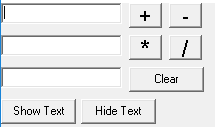
\includegraphics[scale=1]{images/a}\\
\end{center}
\begin{center}
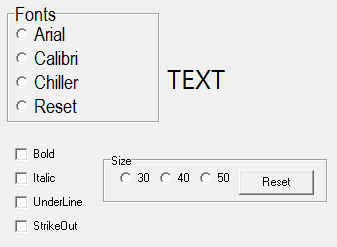
\includegraphics[scale=1]{images/a1}\\
\end{center}

b)Pentru elaborarea subpunctului b am folosit : Ttimer.\\
\begin{center}
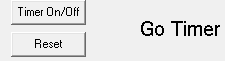
\includegraphics[scale=1]{images/b}\\
\end{center}

c)Pentru elaborarea subpunctului c am folosit : TpaintBox (Bargraf și Diagrama).\\
\begin{center}
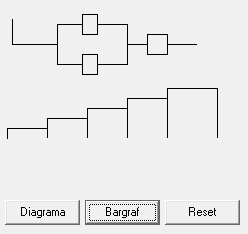
\includegraphics[scale=1]{images/c}\\
\end{center}

\subsection{Linkul la repozitoriul Github}
\begin{center}
\url{https://github.com/dmitrii724/MIDPS}
\end{center}

\subsection{Imagini}
Combinarea tuturor sarcinilor propuse intr-o singura fereastra:\\
\begin{center}
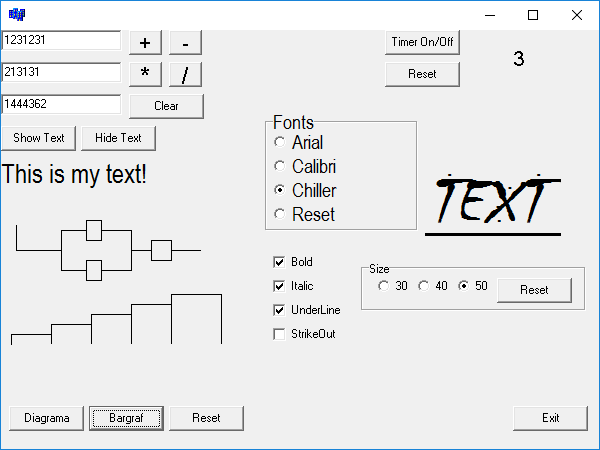
\includegraphics[scale=1]{images/d}\\
\end{center}

\clearpage